% !TeX spellcheck = en_US
%\chapter{Making Dynamic Sexual Contacts Network and adding Vaccination Campaigns}\label{DinamicaYVacunacion}
\chapter{Including new features into the model: Dynamic LSP network and vaccination campaigns}\label{DinamicaYVacunacion}
%\section{Including new features into the model: Dynamic LSP network and vaccination campaigns}
\section{Introducing age and LSP dynamics into the LSP model}
The computational model presented so far is static, that is, once we have assigned the LSPs, they do not change over the time and the nodes do not increase their age. We modulate the possibility of a contagion introducing global probabilities that determine if the existence of a LSP implies sexual intercourses in a given time step per age group $14-17$, $18-29$, $30-39$ and $40-65$. Also, note that the available data about LSPs come from $2003$ and the data of prevalence appears in a study (CLEOPATRA \cite{castellsague2012prevalence}) conducted in $2007-2008$. The sexual behavior has changed in the last $10-15$ years and we would like to include it in our model in some way. Nevertheless, newer data about LSPs and prevalence in Spain are not available.

Thus, in order to introduce age and LSP assignation dynamics in a simple way, we are going to \textit{move} the available data over the time. Figure \ref{fig:dinam1} shows the constant age distribution that do not varies over the time.

\begin{figure}[h!]
	\centering
	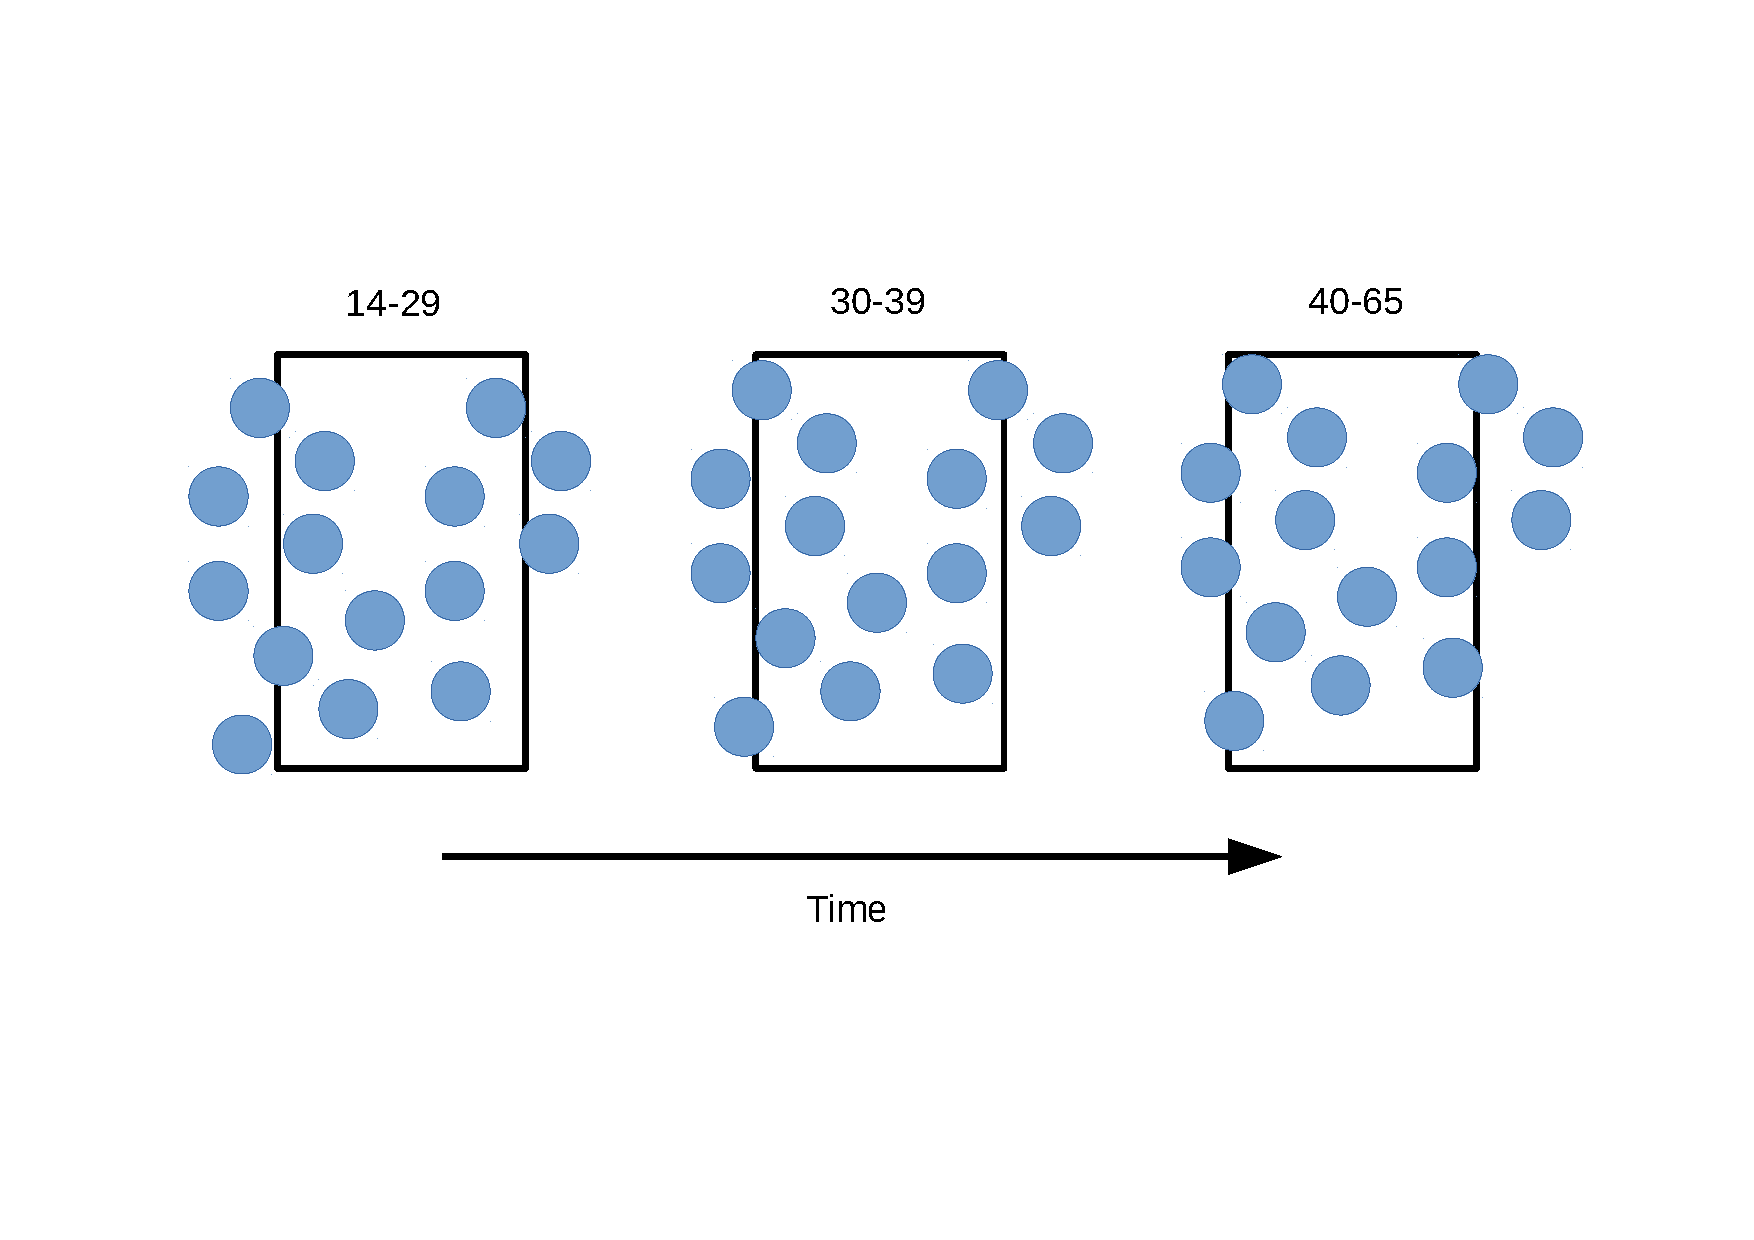
\includegraphics[width=0.7\linewidth]{IMGs/2.-New_features/Dinam_1.pdf}
	\caption{Static LSP network. The ages remain constant over the time. The time only affects the HPV contagion/clearing dynamics.}
	\label{fig:dinam1}
\end{figure}

Then, we evolve the ages of the nodes over the time. As long as the nodes do not change the age group, there is nothing to do. However, how do we \textit{recycle} the nodes that turn 64? And how do we transform the nodes in the first age group $14-29$ when they turn 30?  

To answer the first question, we propose to

\begin{itemize}
	\item preserve its sex in order to maintain the proportion males/females, 
	\item assign $14$ years old to the node, erase all its LSPs and transform it in susceptible,
	\item assign new LSPs according to the LSPs of the age group $14-29$ following the assortativity property.
\end{itemize}

To answer the second question, we propose to

\begin{itemize}
	\item preserve its sex and the infectious state, 
	\item erase all its LSPs and assign new LSPs according to the LSPs of the age group $30-39$ following the assortativity property.
\end{itemize}

This way, as time goes on, we will have the LSP structure by ages as we can see in the Figure \ref{fig:dinam2}.

\begin{figure}[h!]
	\centering
	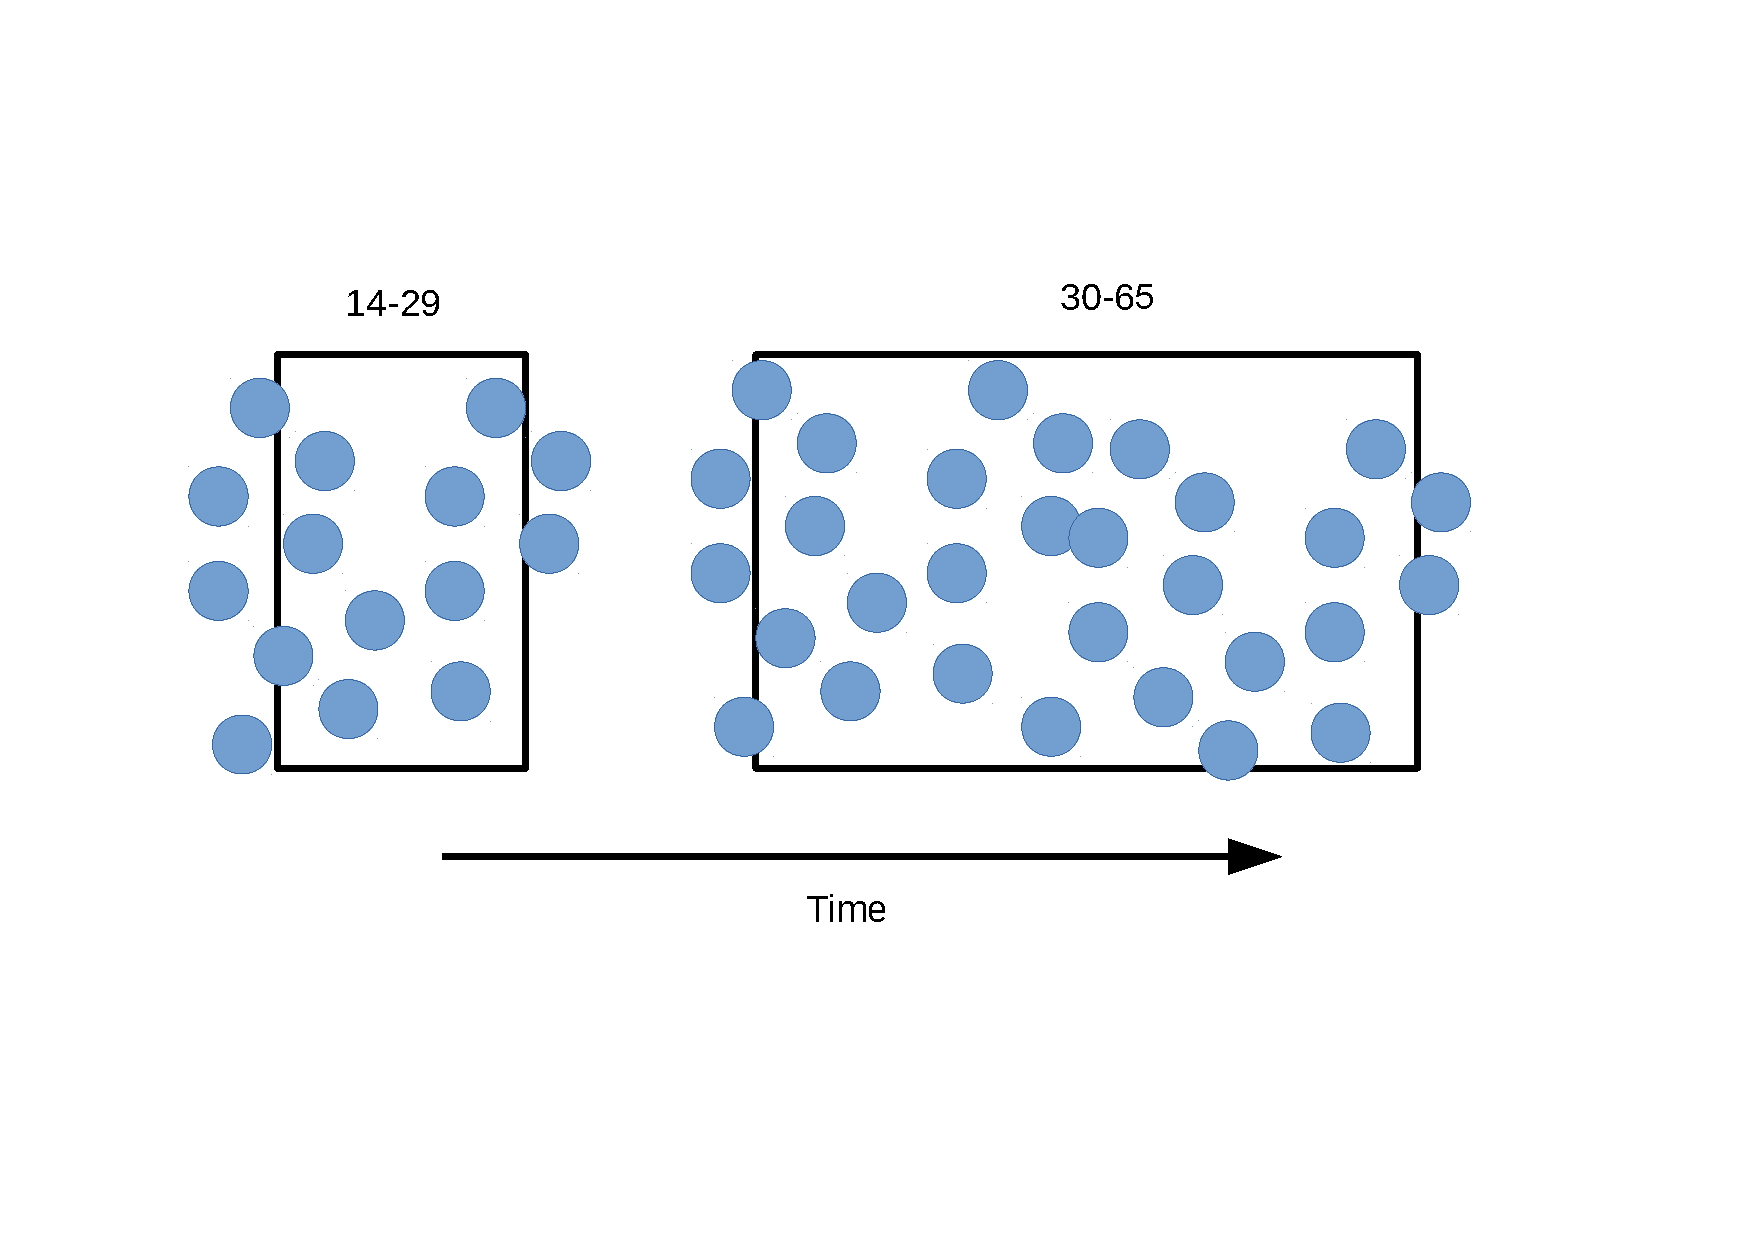
\includegraphics[width=0.7\linewidth]{IMGs/2.-New_features/Dinam_2.pdf}
	\caption{Dynamic LSP network. The ages evolve over the time. The age group 40-65 and their sexual behavior disappear when people grow.}
	\label{fig:dinam2}
\end{figure}

If the node is MSM (male who have sex with males), we perform the above procedure taking into account the division of age groups given in \cite{Durex2002}, $14-19$, $20-24$, $25-29$, $30-39$, $40-49$, $50-59$ and $60-64+$.

Taking into account that the global number of LSP in the age groups $40-64$ is less that in the age group $30-39$, as the time goes on, the global number of LSP in the whole network will increase and the transmission of HPV will also increase. However, the proposed approach may be considered as very conservative because the sexual behavior change in the last $10-15$ years seems to result in an increase of the sexual intercourses greater than the number that we can approach with the proposed dynamic network. Nevertheless, the lack of data do not allow us to quantify the mentioned change.

%, but we take advantage of the static model building and the calibrated model parameters. Furthermore, as we mentioned before, we do not have recent data about sexual behavior in Spain.

\section{When should we start the vaccination campaign?} 
When a realization executes, we use $500$ months to stabilize the static network, then, we change to a dynamic network. Thus, a key point arises and it is to decide in which time instant starts the vaccination schedule. We have performed a simulation with the selected $30$ sets of parameters with $2300$ months (around $191.6$ years) where the network turns dynamic from the month $500$. In the Figure \ref{fig:Estudio_ciclos} we can see the levels of prevalence predicted by the model for 18-64 years old men and women for HR and LR, over the next years.

\begin{figure}[h!]
	\centering
	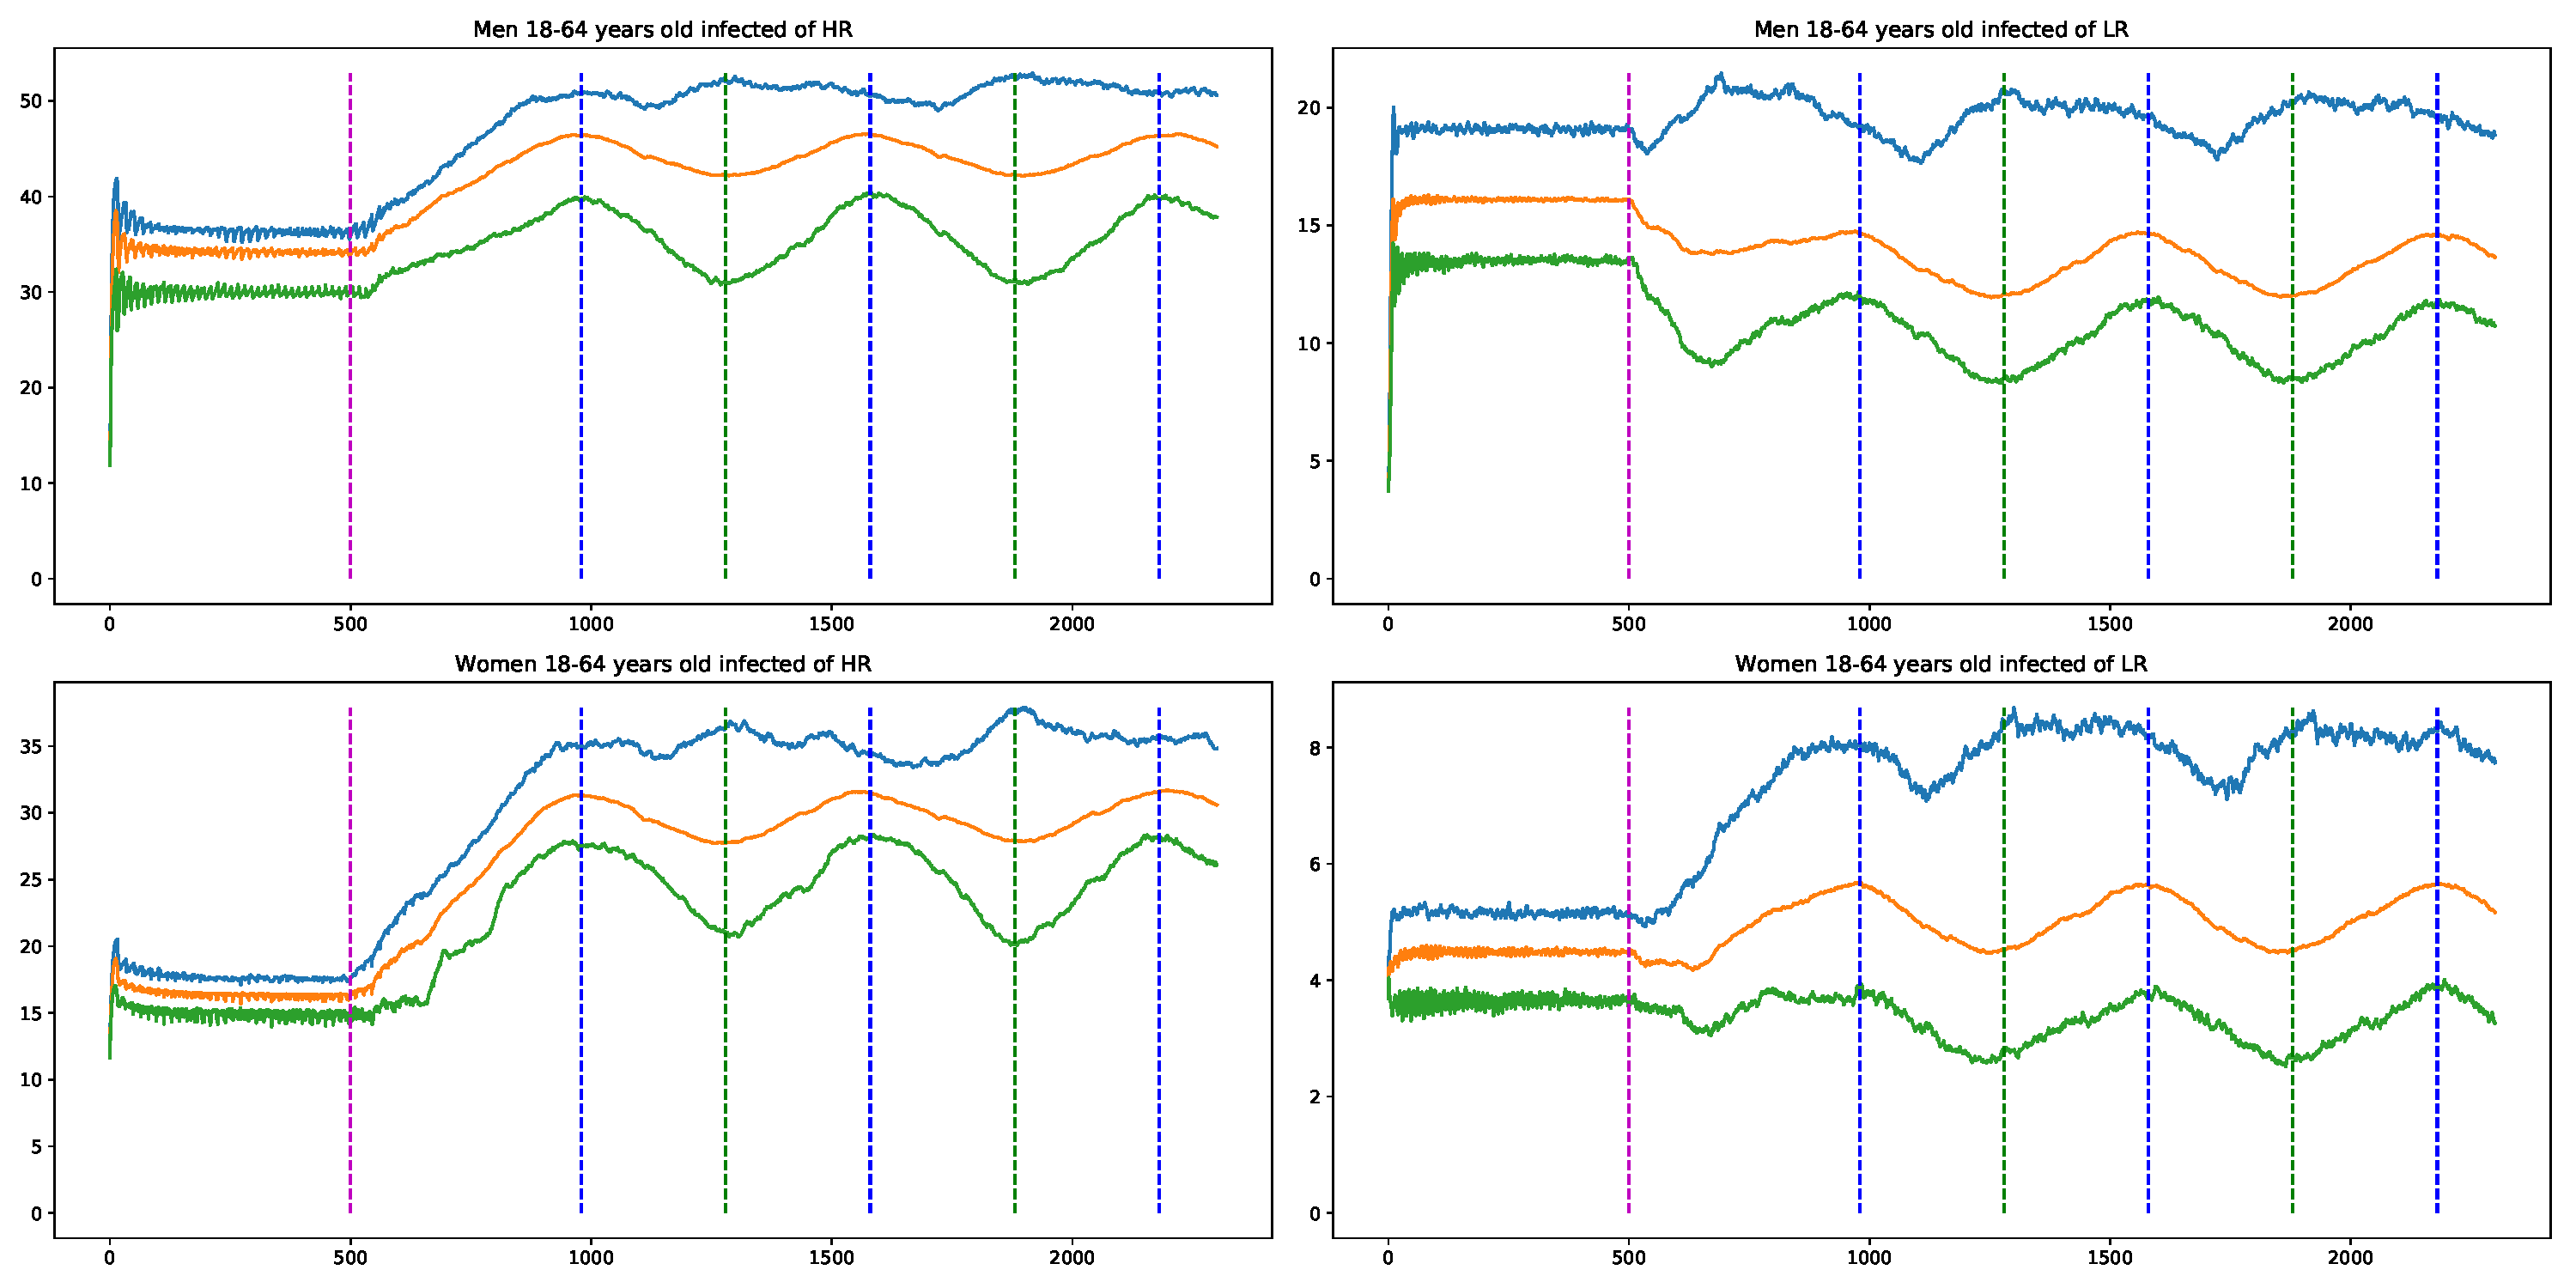
\includegraphics[width=\linewidth]{IMGs/2.-New_features/Estudio_ciclos.pdf}
	\caption{Mean and $95\%$ confidence intervals of the prevalence for 18-64 men and women for HR and LR. Vertical dashed lines indicate milestones of interest. Note the oscillations of the prevalence levels. The blue and green vertical lines correspond to the peaks and valleys of the oscillations. The magenta line, points the month 500 when dynamic network starts.}
	\label{fig:Estudio_ciclos}
\end{figure}

The Figure \ref{fig:Estudio_ciclos} shows the mean and $95\%$ confidence intervals of the $30$ simulations for the prevalence of men and women for HR and LR. The horizontal axis indicates the month and the vertical axis the percentage of infected. As it can be seen, there are oscillation in the evolution of the prevalence.

The vertical lines correspond to:
\begin{itemize}
	\item magenta: month $500$, the static network turns dynamic;
	\item blue: months $980$, $1580$ and $2180$, point out the peaks in the oscillations in the means and the percentiles. Between them, there are $600$ months ($50$ years), the time of a complete generation in the model;
	\item green: months $1280$  and $1880$, point out the valleys. Between the valleys there are also $50$ years, and $25$ years between a peak and a valley. 	
\end{itemize}

In some test executions with vaccination, we have observed that, if we start the vaccination schedule when the prevalence is in the decreasing part (towards a valley) of the oscillation, the herd immunity appears very much sooner than when we start the vaccination schedule in the increasing part (towards a peak).

If we take into account that in the paper \cite{ali2013genital}, the authors reports extraordinary results in Australia, where two years after the vaccine was introduced, the proportion of genital warts diagnosed declined by a $59\%$ in vaccine eligible young women aged 12--26 years in $2007$, and by $39\%$ in men of the same age, we conjecture that, if there are oscillations in the prevalence of HPV over the time, they have taken advantage of a decreasing part of an oscillation.

Recall that our goal is to determine the appropriate month where the vaccination schedule starts, trying to save computations and favoring the apparition of the herd immunity effect as soon as possible, in order to minimize the opposite effect when the oscillation is in the increasing trend if we have vaccinated a large enough number of individuals.

The oscillations in all the cases, men, women, HR and LR, are very similar, as we can see in the Figure \ref{fig:Estudio_ciclos}, except, maybe in some upper percentiles. Also, there are similarities from the first peak, in valleys and peaks. Therefore, in order to take the maximum advantage of the decreasing trends and to save computation, we are going to select the earliest peak, the month $980$, as the starting point for the vaccination.

\section{Introducing vaccination} 
For our simulations, we are going to consider the vaccine GARDASIL9 \cite{gardasil9}. GARDASIL9 is a vaccine indicated in girls and women 9 through 45 years of age for the prevention of  cervical, vulvar, vaginal, and anal cancer caused by HPV types 16, 18, 31, 33, 45, 52, and 58,  genital warts caused by HPV types 6 and 11, and precancerous or dysplastic lesions caused by above HPV types. It is also indicated in boys and men 9 through 45 years of age for the prevention of anal cancer caused by HPV types 16, 18, 31, 33, 45, 52, and 58, genital warts caused by HPV types 6 and 11, and precancerous or dysplastic lesions caused by above HPV types.

The HPV types 6/11 are LR and the remainder (16, 18, 31, 33, 45, 52, and 58) are HR. Thus, GARDASIL9 prevents against $90\%$ of genital wart cases and $90\%$ of the cancer cases \cite{Hartwig2015}. Although GARDASIL9 may prevent partially against other HPV types, for modeling purposes we assume that it does not happen. Therefore, it would be interesting to introduce changes in order to monitor if a node is infected by HPV types included in GARDASIL9 or not, and then, to simulate accurately the prevention effect of the vaccine.

Following the study conducted in \cite{castellsague2012prevalence}, if a woman is infected by HPV LR, the probability to be only infected by 6/11 is $34.23\%$, $63.06\%$ only infected by others than 6/11 and $2.70\%$ to be infected by both. Also, if a woman is infected by HPV HR, the probability to be infected only by 16/18/31/33/45/52/58 is $30.44\%$, $23.66\%$ only infected by others than 16/18/31/33/45/52/58 and $45.90\%$ by both. Due to the lack of information about men, we will also use the above percentages for men.

Then, before starting the vaccination, we label men and women as infected of HPV LR 6/11 or infected of HPV LR other than 6/11 or infected of both, following the above percentages. Analogously, we label men and women as infected of HPV HR 16/18/31/33/45/52/58 or infected of HPV HR other than 16/18/31/33/45/52/58 or infected of both.

Once these assignments are done, we continue with the HPV transmission dynamics including the vaccination, taking into account the new labels we included. If a node has been vaccinated, it can be infected by the types of HPV different to those that GARSDASIL9 prevents and, in this case, they will never be infected of 6/11 nor 16/18/31/33/45/52/58. If a node has not been vaccinated, can be infected by any HPV type. 

The assumed effectiveness of the vaccine is $96.5\%$.

\section{Introducing vaccination loss protection}
In the previous section we assume that the protection of GARDASIL9 is forever. In fact, until now, people vaccinated by GARDASIL (previous version of GARDASIL9) do not have experienced any loss in the protection. But this does not mean that it could happen in the future. 

In fact, we want to simulate the worst possible scenario, that is, the sudden drop to zero of the protection. To simulate this possibility, we will introduce a new parameter that represents the time after the vaccination where the protection is complete. Therefore, after this time, the vaccinated individual will behave as a non-vaccinated individual.

\section{Introducing variations in the vaccination coverage}
One of our goals is to simulate scenarios where variations in the vaccination coverage have been occurred and we want to study the effect in the global protection against HPV due to these variation of the coverage. To simulate these scenarios, we will include into the model vectors of coverage, indicating the vaccine coverage every month, and vaccinating the people following these variable coverages. 
